\documentclass[12pt, a4paper]{report}

\usepackage{graphicx}
\usepackage{fancyhdr}
\usepackage{subcaption}
\usepackage{lipsum}
\usepackage{setspace}
\usepackage[hidelinks]{hyperref}
\usepackage[left=1.25in, right=1in, top=0.75in, bottom=0.75in]{geometry}
\usepackage{mathptmx}
\usepackage[numbers]{natbib}
\usepackage{emptypage}
\usepackage[nottoc, notlof]{tocbibind}
\renewcommand{\bibname}{REFERENCES}
\usepackage{enumitem}
\usepackage{tikz}
\usetikzlibrary{positioning,arrows.meta,shapes.geometric,fit, calc}
\usepackage{graphicx}\graphicspath{{img/}}
\usepackage{xcolor}
\usepackage{titlesec}
\usepackage{booktabs}
\usepackage{array}
\usepackage{dirtree}
\usepackage{caption}
\usepackage{float}
\usepackage{tabularx}
\usepackage{listings}

% --- PACKAGES FOR NUMBERING ---
\usepackage{chngcntr} 

\lstset{
	basicstyle=\small\rmfamily,
	columns=fullflexible,   % changing to fullflexible handles spaces better in text fonts
	breaklines=true,
	showstringspaces=false, % This removes the black squares/markers in strings
	keepspaces=true         % This ensures indentation spaces aren't collapsed
}

% Adjust Chapter Spacing
\titleformat{\chapter}[display]
{\normalfont\huge\bfseries}{\raggedright\chaptertitlename\ \thechapter}{5pt}{\centering\Huge}
\titlespacing*{\chapter}{-9pt}{-40pt}{15pt}

% --- TOC AND LOF SETTINGS ---
\usepackage{tocloft}

% 1. Space adjustments
\setlength{\cftbeforetoctitleskip}{-1em} 
\setlength{\cftaftertoctitleskip}{10pt} 
\setlength{\cftbeforeloftitleskip}{-1em}
\setlength{\cftafterloftitleskip}{10pt}

% 2. REMOVE DOTS
\renewcommand{\cftsecdotsep}{\cftnodots}
\renewcommand{\cftsubsecdotsep}{\cftnodots}
\renewcommand{\cftfigdotsep}{\cftnodots}

% 3. CHANGE FIGURE NUMBERING HIERARCHY (The fix)
% Keep the reset at subsection level
\counterwithin{figure}{subsection} 

% 4. INTELLIGENT LABELING
% This removes the ".0." if you are not inside a subsection
\renewcommand{\thefigure}{%
	\ifnum\value{subsection}=0
	\thesection.\arabic{figure}%      -> Prints 6.1.1
	\else
	\thesubsection.\arabic{figure}%   -> Prints 4.3.1.1
	\fi
}

% 5. ADJUST LIST OF FIGURES INDENTATION
\setlength{\cftfignumwidth}{4.5em} 

% -----------------------------------

\setcounter{secnumdepth}{3}
\setcounter{tocdepth}{3}

% Page style setup
\pagestyle{fancy}
\fancyhf{}
\setlength{\headheight}{30pt}
\definecolor{burgundy}{RGB}{128,0,32}
\renewcommand{\headrulewidth}{2pt}
\renewcommand{\footrulewidth}{2pt}
\renewcommand{\headrule}{\hbox to\headwidth{\color{burgundy}\leaders\hrule height \headrulewidth\hfill}}
\renewcommand{\footrule}{\hbox to\headwidth{\color{burgundy}\leaders\hrule height \footrulewidth\hfill}}
\fancyhead[L]{Brain Decoding system using fMRI Data and Deep learning}
\fancyhead[C]{}
\fancyfoot[L]{Dept. of CSE, AITM, Belagavi}
\fancyfoot[R]{\thepage}

% Redefine plain style for chapter first pages
\fancypagestyle{plain}{
	\fancyhf{}
	\fancyhead[L]{Brain Decoding system using fMRI Data and Deep learning}
	\fancyhead[C]{}
	\fancyfoot[L]{Dept. of CSE, AITM, Belagavi}
	\fancyfoot[R]{\thepage}
	\renewcommand{\headrulewidth}{2pt}
	\renewcommand{\footrulewidth}{2pt}
	\renewcommand{\headrule}{\hbox to\headwidth{\color{burgundy}\leaders\hrule height \headrulewidth\hfill}}
	\renewcommand{\footrule}{\hbox to\headwidth{\color{burgundy}\leaders\hrule height \footrulewidth\hfill}}
}

\begin{document}
	
	% Front matter with Roman numerals
	\pagenumbering{roman}
	
	% Generate table of contents
	\begin{singlespace}
		\tableofcontents
	\end{singlespace}
	\newpage
	
	% Generate list of figures
	\begin{singlespace}
		\listoffigures
	\end{singlespace}
	\newpage
	
	% Start Double Spacing for the actual content
	\doublespacing
	
	% Abstract
	\thispagestyle{empty}
	\begin{center}
		\large\textbf{ABSTRACT}
	\end{center}
	\vspace{0.5cm}
	
	Brain decoding from functional Magnetic Resonance Imaging (fMRI) represents a transformative approach in cognitive neuroscience for understanding neural mechanisms underlying human emotions. This work presents a deep learning-based brain decoding system that automatically recognizes emotional states from fMRI recordings. A convolutional neural network (CNN) architecture specifically designed for functional connectivity matrix classification, integrating features from three complementary brain parcellation atlases (Harvard-Oxford, AAL, and Destrieux). The deep learning model processes connectivity patterns as 2D images, learning hierarchical representations directly from data. Validation on the ds003548 emotional faces dataset containing 16 subjects and four emotion categories demonstrates that our CNN-based brain decoding system achieves 84\% classification accuracy, significantly outperforming traditional machine learning approaches (68-76\% accuracy). The deep learning framework automatically discovers discriminative connectivity patterns without manual feature engineering, with Leave-One-Subject-Out cross-validation confirming robust generalization to unseen individuals. Results establish deep learning as a superior approach for brain decoding applications, with implications for brain-computer interfaces, affective disorder diagnosis, and cognitive neuroscience research.
	
	\textbf{Keywords:} brain decoding, deep learning, fMRI analysis, convolutional neural networks, emotion recognition, functional connectivity
	
	\clearpage
	
	% Main content with Arabic numerals
	\pagenumbering{arabic}
	
	% Include your chapters
	\nocite{ref1,ref2,ref3,ref4,ref5,ref6,ref7,ref8}
	\chapter{INTRODUCTION}

\section{Overview of Functional Magnetic Resonance Imaging (fMRI)}

\hspace{0.5cm}Functional Magnetic Resonance Imaging (fMRI) represents a revolutionary non-invasive neuroimaging technique that has transformed our understanding of human brain function since its development in the early 1990s. Unlike structural MRI which captures static anatomical information, fMRI measures dynamic brain activity by detecting changes in blood oxygenation levels associated with neural activity, a phenomenon known as the Blood-Oxygen-Level-Dependent (BOLD) signal.

The fundamental principle underlying fMRI is neurovascular coupling when neurons in a particular brain region become active, they require increased oxygen and glucose to support their metabolic demands. The brain responds by increasing blood flow to these active regions, delivering oxygen-rich hemoglobin. Since oxygenated and deoxygenated hemoglobin possess different magnetic properties, this localized change in blood oxygenation creates detectable alterations in the MRI signal. Modern fMRI scanners can capture these hemodynamic changes with spatial resolution of 2-3 millimeters and temporal resolution of 1-3 seconds, enabling researchers to observe which brain regions activate during specific cognitive, perceptual, or emotional processes.

fMRI has become the dominant tool in cognitive neuroscience research due to several key advantages. First, it provides whole-brain coverage, allowing simultaneous observation of distributed neural networks rather than isolated brain regions. Second, unlike Positron Emission Tomography (PET), fMRI does not require radioactive tracers, making it safe for repeated measurements on the same individuals. Third, the non-invasive nature permits studies of healthy populations across diverse age ranges and clinical conditions. These capabilities have enabled groundbreaking discoveries about brain organization, from mapping the default mode network during rest to revealing neural circuits underlying memory, attention, and emotion processing.

In the context of emotion research, fMRI has proven particularly valuable for identifying brain networks involved in affective processing. Traditional lesion studies and electrophysiology provided limited spatial coverage, while fMRI enables comprehensive mapping of emotion-related activations across cortical and subcortical structures. Researchers have used fMRI to demonstrate that emotions engage distributed networks involving the amygdala for salience detection, prefrontal cortex for regulation and appraisal, insula for interoceptive awareness, and anterior cingulate for conflict monitoring. These findings have shifted emotion theories away from localizationist models proposing dedicated emotion centers toward network-based frameworks emphasizing interactions across multiple brain systems.

However, fMRI data also presents substantial analytical challenges. Each scanning session generates high-dimensional datasets containing millions of voxel time series, creating a "curse of dimensionality" problem where the number of features vastly exceeds the number of observations. The BOLD signal exhibits low signal-to-noise ratio, requiring sophisticated preprocessing to remove physiological noise from cardiac and respiratory cycles, head motion artifacts, and scanner drift. Additionally, the hemodynamic response peaks 4-6 seconds after neural activity, introducing temporal lag between cognitive events and measured signals. These complexities necessitate advanced analytical approaches capable of extracting meaningful patterns from noisy, high-dimensional neuroimaging data-motivating the application of machine learning and deep learning techniques to fMRI analysis.

\section{Machine Learning Approaches in fMRI Analysis}

\hspace{0.5cm}The application of machine learning to fMRI analysis represents a paradigm shift from traditional univariate statistical methods toward multivariate pattern recognition approaches. Classical fMRI analysis employed General Linear Models (GLM) and t-tests to identify individual voxels showing significant activation differences between experimental conditions. While effective for localization, these mass-univariate methods discard information about spatial patterns and inter-voxel relationships, limiting their sensitivity for detecting distributed neural representations.

Machine learning methods, in contrast, leverage patterns across multiple voxels simultaneously, enabling decoding of mental states from distributed brain activity. The fundamental premise of brain decoding is that specific cognitive or emotional states correspond to characteristic spatial patterns of neural activity that machine learning classifiers can learn to recognize. Rather than asking "which brain regions activate during emotion X?", decoding approaches ask "can we identify which emotion a person is experiencing based on their brain activity pattern?" This predictive framework naturally aligns with machine learning's supervised learning paradigm.

Support Vector Machines (SVMs) emerged as the dominant classical approach for fMRI classification due to their effectiveness with high-dimensional data. SVMs construct optimal hyperplanes that maximally separate different classes in feature space, with kernel functions enabling nonlinear decision boundaries. The regularization inherent in SVMs prevents overfitting even when the number of features (voxels) exceeds the number of samples. Numerous studies have successfully applied SVMs to decode various mental states including visual stimuli categories, memory contents, and emotional experiences. For emotion classification specifically, SVMs typically extract features from anatomically-defined regions of interest or whole-brain voxel patterns, achieving accuracies ranging from 60-75\% for multi-class discrimination.

Random Forests represent another widely-used approach, combining predictions from multiple decision trees trained on bootstrap samples of the data. This ensemble method offers several advantages for neuroimaging: natural handling of high-dimensional inputs, robustness to outliers and noisy features, and built-in feature importance measures that identify which brain regions contribute most to classification. Random Forests have demonstrated competitive performance with SVMs while providing greater interpretability through feature importance rankings. Studies applying Random Forests to emotion decoding have revealed that limbic-prefrontal connections and default mode network patterns carry substantial discriminative information.

Logistic Regression, despite its simplicity, remains valuable as an interpretable baseline. L2-regularized logistic regression learns linear weights for each feature, enabling direct interpretation of which brain regions positively or negatively contribute to each emotion category. While typically achieving lower accuracy than nonlinear methods, logistic regression's transparency makes it useful for hypothesis testing and comparison against more complex models.

Beyond classification, machine learning has enabled novel analyses of fMRI data including representational similarity analysis, dimensionality reduction through Principal Component Analysis and Independent Component Analysis, and functional connectivity estimation. Connectivity analysis examines statistical relationships between regional time series, revealing network organization underlying cognitive functions. Pearson correlation between regions provides the simplest connectivity measure, though partial correlation and regularized precision estimation offer more sophisticated approaches accounting for indirect connections.

Despite these successes, classical machine learning methods face inherent limitations when applied to fMRI analysis. First, they typically require manual feature engineering-researchers must decide which brain regions to examine, how to summarize regional activity, and which connectivity measures to compute. This introduces researcher bias and may miss important patterns not anticipated a priori. Second, most classical methods employ shallow architectures with limited capacity for hierarchical representation learning. Complex brain patterns involving interactions across multiple spatial scales may exceed the representational capacity of linear or single-layer nonlinear models. Third, classical approaches struggle with very small sample sizes typical in neuroimaging studies (10-30 subjects), as they cannot leverage the temporal structure of fMRI time series to augment effective sample size.

These limitations motivated exploration of deep learning approaches that can automatically learn hierarchical feature representations directly from neuroimaging data, eliminating manual feature engineering while capturing complex nonlinear patterns that classical methods miss, thus promising more robust and accurate diagnostic and prognostic models. This transition leverages the power of convolutional and recurrent networks to discern subtle, clinically relevant biomarkers hidden within high-dimensional imaging datasets, significantly enhancing the potential for personalized medicine and early detection of neurological disorders, by offering a data-driven pathway to understand brain pathology. The capacity of deep learning to handle the inherent noise and variability in clinical data makes it an increasingly indispensable tool for translating raw scanner output into actionable insights.
\section{Deep Learning for Emotion Recognition in Brain Decoding}

\hspace{0.5cm}Deep learning has revolutionized computer vision, natural language processing, and speech recognition through its capacity to automatically learn hierarchical representations from raw data. Unlike classical machine learning requiring handcrafted features, deep neural networks discover increasingly abstract features through multiple processing layers from simple edges in early layers to complex object parts in intermediate layers to semantic concepts in deep layers. This automatic feature learning has proven transformative across domains, motivating its application to neuroimaging analysis including emotion recognition from fMRI.

Convolutional Neural Networks (CNNs), originally developed for image analysis, have emerged as a natural architecture for processing fMRI data. CNNs exploit spatial structure through convolutional layers that apply learnable filters across the input, detecting local patterns while sharing parameters to reduce model complexity. For fMRI analysis, brain activity patterns and connectivity matrices can be represented as structured 2D or 3D images amenable to convolutional processing. Several key architectural components make CNNs particularly suitable for neuroimaging: convolutional layers capture local spatial patterns, pooling layers provide translation invariance and spatial downsampling, batch normalization stabilizes training dynamics, dropout prevents overfitting, and fully-connected classification layers map learned features to emotion categories.

Recent studies have begun applying CNNs to fMRI-based emotion recognition with promising results. Early approaches processed whole-brain activation maps as 3D volumes, using 3D convolutions to detect spatial patterns across voxels. However, these methods face challenges from the extremely high dimensionality of volumetric fMRI data (often 100,000+ voxels) and small sample sizes typical in neuroimaging studies. More recent work has focused on functional connectivity matrices representing pairwise correlations between brain regions, which can be treated as 2D images with spatial structure reflecting anatomical relationships between connections.

The application of CNNs to connectivity matrices offers several advantages over classical approaches. First, CNNs automatically learn which connections and connection patterns discriminate emotions, eliminating the need for manual feature selection based on prior hypotheses. Second, hierarchical feature learning enables discovery of multi-scale patterns from individual connections in early layers to network motifs in intermediate layers to whole-brain configurations in deep layers. Third, CNNs naturally capture nonlinear relationships and interactions between features that linear models cannot represent. Fourth, weight sharing through convolution dramatically reduces the number of parameters compared to fully-connected networks, providing regularization that helps prevent overfitting on small datasets.

Despite their promise, applying deep learning to fMRI emotion recognition presents substantial technical challenges. The primary challenge is small sample size: while CNNs excel with millions of training examples in computer vision, neuroimaging studies typically include only 10-30 subjects due to scanning costs and time constraints. This creates severe risk of overfitting where models memorize training examples rather than learning generalizable patterns. Researchers have addressed this through several strategies: aggressive regularization using high dropout rates (25-50\%) and L2 weight penalties data augmentation through temporal windowing that generates multiple samples per experimental run; transfer learning where models pre-trained on large resting-state fMRI datasets are fine-tuned for emotion tasks and architecture design favoring parameter efficiency through global average pooling rather than large fully-connected layers.

A second challenge involves ensuring subject-independent generalization. Clinical and commercial applications require models that perform well on completely novel individuals not seen during training. However, substantial inter-subject variability in brain anatomy, functional organization, and emotional reactivity can cause models to overfit subject-specific idiosyncrasies. Rigorous evaluation through Leave-One-Subject-Out (LOSO) cross-valida-\\tion, where each subject is held out for testing while training on all others, provides unbiased estimates of true generalization performance. Studies employing LOSO validation have demonstrated that well-regularized CNNs can learn emotion representations that generalize across individuals, though performance typically decreases compared to subject-specific models.

A third challenge concerns interpretability: understanding what patterns the network has learned and whether they align with neuroscience knowledge. Techniques such as Grad-CAM (Gradient-weighted Class Activation Mapping) visualize which connections or brain regions most influence predictions by examining gradient flow through the network. Studies applying these visualization methods to emotion-decoding CNNs have found that learned patterns often align with established neuroscience highlighting limbic-prefrontal connections for emotion processing, default mode network for internal states, and attention networks for arousal modulation. This neurobiological plausibility provides confidence that models capture meaningful patterns rather than artifacts.

The integration of multiple brain parcellation atlases represents a particularly promising approach for enhancing CNN performance. Different anatomical atlases (Harvard-Oxford with 48 regions, AAL with 116 regions, Destrieux with 148 regions) provide complementary perspectives on brain organization at varying spatial scales. Coarse atlases capture large-scale network structure, while fine atlases reveal local connectivity patterns. Training separate CNN models on each atlas's connectivity matrices and combining their predictions through ensemble learning leverages this complementary information, improving accuracy beyond single-atlas approaches. This multi-scale integration mirrors the hierarchical organization of the brain itself, where emotion processing involves interactions spanning local circuits to large-scale networks.

Looking forward, deep learning for fMRI emotion recognition continues advancing through several directions. Recurrent neural networks (RNNs) and Long Short-Term Memory (LSTM) networks model temporal dynamics by processing fMRI time series sequentially, capturing evolving connectivity patterns during emotional episodes. Graph neural networks incorporate brain network topology explicitly, learning representations that respect anatomical structure. Attention mechanisms enable models to dynamically focus on relevant brain regions for each emotion category. Multi-modal integration combines fMRI with EEG for temporal precision, physiological signals for bodily state, and behavioral measures for comprehensive emotion assessment.

These advances position deep learning as a transformative technology for brain decoding applications. By achieving superior accuracy through automatic feature learning, capturing complex patterns beyond classical methods' reach, and scaling effectively as neuroimaging datasets grow, deep learning systems promise to accelerate neuroscience research, enable objective clinical diagnostics for affective disorders, and power next generation brain-computer interfaces for emotion-aware technology. This project contributes to this vision by developing a CNN-based system integrating multi-atlas connectivity for robust emotion recognition from fMRI data.
	\chapter{LITERATURE SURVEY}

\noindent
\textbf{Title: } Inter-Subject Transfer Learning for Generalizable fMRI Emotion Decoding \textbf{\cite{ref1}} \\
\textbf{Authors:} D. P. Sharma, K. L. Nguyen, S. T. Perez \\
\textbf{Journal:} Biological Psychiatry (2025) \\
\textbf{Summary:} This paper addresses the significant challenge of \textbf{inter-subject variability} inherent in fMRI data by implementing a robust \textbf{Transfer Learning} framework. The approach, which utilizes \textbf{Domain Adversarial Neural Networks (DANN)}, focuses on decoupling subject-specific noise from genuine emotional activation patterns. It achieves higher \textbf{generalization accuracy} when applying models trained on one group of subjects to a completely new, unseen group, which is essential for establishing the model's clinical and research reliability.

\vspace{1.5em}

\noindent
\textbf{Title:} Real-Time Emotion Recognition from Whole-Brain fMRI using 3D Convolutional Neural Networks \textbf{\cite{ref2}} \\
\textbf{Authors:} J. M. Smith, L. K. Johnson, R. B. Chen \\
\textbf{Journal:} NeuroImage (2024) \\
\textbf{Summary:} This study proposes a method for real-time decoding of basic emotional states from fMRI BOLD signals by employing a \textbf{3D Convolutional Neural Network (3D-CNN)}. The system is designed to analyze whole-brain fMRI volumes directly, demonstrating improved spatial feature extraction compared to traditional Region-of-Interest (ROI) based analysis. It achieves high classification accuracy on emotional movie clip datasets and emphasizes maintaining the low latency crucial for effective real-time neuro-feedback applications.

\vspace{1.5em}

\noindent
\textbf{Title: } Spatio-Temporal Fusion Network for Dynamic fMRI-based Affective State Classification \textbf{\cite{ref3}} \\
\textbf{Authors:} H. Liu, C. Wang, G. Z. Khan \\
\textbf{Journal:} IEEE Transactions on Affective Computing (2024) \\
\textbf{Summary:} This research introduces a \textbf{hybrid deep learning network} that combines \textbf{3D-CNNs} for spatial feature extraction and \textbf{Long Short-Term Memory (LSTM)} units for temporal sequence modeling. The network's design effectively captures both the static patterns of brain activation and the dynamic, time-varying nature of emotional responses. It successfully classifies the continuous \textbf{valence} and \textbf{arousal} dimensions of emotion, highlighting the importance of explicitly modeling the temporal evolution of brain states.

\vspace{1.5em}


\noindent
\textbf{Title: } Semantic reconstruction of continuous language from non-invasive brain recordings \textbf{\cite{ref5}} \\
\textbf{Authors:} Tang, J., LeBel, A., Jain, S., \& Huth, A. G. \\
\textbf{Journal:} Nature Neuroscience (2023) \\
\textbf{Summary:} Used an encoding model based on GPT-1 (Transformer) to predict fMRI responses to natural language. A beam search decoder then generated text candidates that best matched the recorded brain activity.

\vspace{1.5em}

\noindent
\textbf{Title: } High-resolution image reconstruction with latent diffusion models from human brain activity \textbf{\cite{ref6}} \\
\textbf{Authors:} Takagi, Y., \& Nishimoto, S. \\
\textbf{Journal:} CVPR (2023) \\
\textbf{Summary:} Integrated fMRI signals with Stable Diffusion (Latent Diffusion Models). They mapped brain activity from the Early Visual Cortex to the model's latent space to control structural features, and higher visual cortex activity to control semantic text embeddings.

\vspace{1.5em}

\noindent
\textbf{Title: } Deep image reconstruction from human brain activity \textbf{\cite{ref7}} \\
\textbf{Authors:} Shen, G., Dwivedi, K., Majima, K., Horikawa, T., \& Kamitani, Y. \\
\textbf{Journal:} PLOS Computational Biology (2019) \\
\textbf{Summary:} Used a \textbf{Deep Generator Network (DGN)} and a Deep Neural Network (VGG-19) to translate fMRI activity into hierarchical image features. They optimized pixel values iteratively to match the predicted DNN features.

\vspace{1.5em}
\noindent
\textbf{Title: } Toward a universal decoder of linguistic meaning from brain activation \textbf{\cite{ref8}} \\
\textbf{Authors:} Pereira, F., Lou, B., Pritchett, B., et al. \\
\textbf{Journal:} Nature Communications (2018) \\
\textbf{Summary:} Utilized a Ridge Regression model combined with global semantic vectors (GloVe) and a Universal Sentence Encoder. This approach mapped fMRI patterns to a high-dimensional semantic space.

\vspace{1.5em}
\noindent
\textbf{Title:} Decoding the Nature of Emotion in the Brain \textbf{\cite{kragel2016}} \\
\textbf{Authors:} Philip A. Kragel, Kevin S. LaBar \\
\textbf{Journal:} Trends in Cognitive Sciences (2016) \\
\textbf{Summary:} This comprehensive review examines the neural mechanisms underlying emotion decoding, evaluating evidence for both \textbf{discrete} and \textbf{dimensional} models of emotion representation in the brain. The authors discuss advances in \textbf{multivariate pattern analysis (MVPA)} techniques that enable identification of distributed neural patterns associated with specific emotional states. The paper emphasizes how machine learning approaches have revealed that emotions are represented through complex, distributed networks rather than isolated brain regions, challenging traditional locationist views of emotional processing.

\vspace{1.5em}

\noindent
\textbf{Title:} Discrete Neural Signatures of Basic Emotions \textbf{\cite{saarimaki2016}} \\
\textbf{Authors:} Heini Saarimäki, Athanasios Gotsopoulos, Iiro P. Jääskeläinen, Jouko Lampinen, Patrik Vuilleumier, Riitta Hari, Mikko Sams, Lauri Nummenmaa \\
\textbf{Journal:} Cerebral Cortex (2016) \\
\textbf{Summary:} This neuroimaging study utilized \textbf{machine learning classifiers} to identify distinct neural patterns associated with six basic emotions (anger, fear, disgust, happiness, sadness, and surprise). The research demonstrates that each emotion generates a unique, \textbf{spatially distributed activation pattern} across multiple brain regions including the limbic system, sensorimotor cortices, and prefrontal areas. Using \textbf{support vector machines (SVM)}, the authors achieved significant above-chance classification accuracy, providing evidence for discrete neural representations of basic emotional categories.

\vspace{1.5em}

\noindent
\textbf{Title:} A Bayesian Model of Category-Specific Emotional Brain Responses \textbf{\cite{wager2015}} \\
\textbf{Authors:} Tor D. Wager, Jian Kang, Timothy D. Johnson, Thomas E. Nichols, Ajay B. Satpute, Lisa Feldman Barrett \\
\textbf{Journal:} PLoS Computational Biology (2015) \\
\textbf{Summary:} This work presents a sophisticated \textbf{Bayesian hierarchical model} for analyzing category-specific brain responses to emotional stimuli across multiple studies. The framework addresses the challenge of identifying consistent neural patterns while accounting for study-level variability and individual differences. The model integrates data from numerous neuroimaging experiments to estimate the probability that specific brain regions are consistently activated during particular emotional experiences, providing a probabilistic approach to understanding emotion-related neural activity.

\vspace{1.5em}

\noindent
\textbf{Title:} Recent Progress and Outstanding Issues in Motion Correction in Resting State fMRI \textbf{\cite{power2015}} \\
\textbf{Authors:} Jonathan D. Power, Bradley L. Schlaggar, Steven E. Petersen \\
\textbf{Journal:} NeuroImage (2015) \\
\textbf{Summary:} This critical review addresses the substantial impact of \textbf{head motion artifacts} on fMRI data quality and the effectiveness of various \textbf{motion correction strategies}. The authors evaluate both prospective and retrospective correction methods, including realignment, scrubbing, and regression-based approaches. The paper provides practical recommendations for preprocessing pipelines, emphasizing that even small amounts of head motion can introduce systematic biases in functional connectivity analyses and classification studies, making rigorous motion correction essential for reliable emotion decoding research.

\vspace{1.5em}

\noindent
\textbf{Title:} Machine Learning for Neuroimaging with Scikit-learn \textbf{\cite{abraham2014}} \\
\textbf{Authors:} Alexandre Abraham, Fabian Pedregosa, Michael Eickenberg, Philippe Gervais, Andreas Mueller, Jean Kossaifi, Alexandre Gramfort, Bertrand Thirion, Gael Varoquaux \\
\textbf{Journal:} Frontiers in Neuroinformatics (2014) \\
\textbf{Summary:} This paper introduces practical applications of the \textbf{Scikit-learn} machine learning library for neuroimaging analysis, demonstrating how standardized ML workflows can be applied to fMRI data. The authors present methodologies for \textbf{feature extraction, dimensionality reduction, and classification} specific to brain imaging data structures. The work includes examples of \textbf{cross-validation strategies} adapted for neuroimaging's unique challenges, such as spatial autocorrelation and temporal dependencies, providing a foundational framework for applying machine learning to emotion decoding tasks.

\vspace{1.5em}

\noindent
\textbf{Title:} Learning and Comparing Functional Connectomes Across Subjects \textbf{\cite{varoquaux2013}} \\
\textbf{Authors:} Gael Varoquaux, R. Cameron Craddock \\
\textbf{Journal:} NeuroImage (2013) \\
\textbf{Summary:} This study addresses the fundamental challenge of \textbf{inter-subject variability} in functional connectivity patterns by developing methods to learn and compare brain network organization across individuals. The authors propose approaches for constructing \textbf{group-level functional connectomes} that capture both common organizational principles and individual differences. The work emphasizes techniques for \textbf{spatial normalization and parcellation} that enable more robust cross-subject analyses, which is particularly relevant for building generalizable emotion decoding models that can be applied to new individuals.

\vspace{1.5em}
\noindent
\textbf{Title:} Identifying Emotions on the Basis of Neural Activation \textbf{\cite{kassam2013}} \\
\textbf{Authors:} Karim S. Kassam, Amanda R. Markey, Vladimir L. Cherkassky, George Loewenstein, Marcel Adam Just \\
\textbf{Journal:} PLoS ONE (2013) \\
\textbf{Summary:} This pioneering study demonstrates that distinct emotional states can be reliably identified from fMRI activation patterns using \textbf{machine learning classification}. Participants experienced nine different emotions while brain activity was recorded, and a \textbf{Gaussian Naive Bayes classifier} successfully distinguished between these emotional states with accuracy significantly above chance level. The research identifies key brain regions contributing to emotion classification, including the \textbf{insula, prefrontal cortex, and anterior cingulate}, establishing feasibility for individual-level emotion decoding from neuroimaging data.

\vspace{1.5em}

\noindent
\textbf{Title:} The Brain Basis of Emotion: A Meta-analytic Review \textbf{\cite{lindquist2012}} \\
\textbf{Authors:} Kristen A. Lindquist, Tor D. Wager, Hedy Kober, Eliza Bliss-Moreau, Lisa Feldman Barrett \\
\textbf{Journal:} Behavioral and Brain Sciences (2012) \\
\textbf{Summary:} This extensive meta-analysis synthesizes findings from over 160 neuroimaging studies to examine whether discrete emotions correspond to distinct neural signatures. The authors challenge the \textbf{locationist hypothesis} that specific brain regions are consistently associated with particular emotion categories. Instead, they propose a \textbf{constructionist framework} where emotions emerge from interactions between domain-general psychological processes implemented in distributed brain networks. The review highlights the complexity of emotion representation and the importance of considering network-level activity rather than isolated regional activations in emotion decoding research.
	\chapter{PROBLEM DEFINITION AND OBJECTIVES}

\section{Problem Definition}
\hspace{0.5cm}Understanding human cognitive states, particularly emotions and the veracity of statements (truth vs. lie), has traditionally been a significant challenge in neuroscience and psychology. Accurate detection of these states is critical for applications ranging from mental health diagnosis to forensic analysis. However, the complexity of the human brain makes it difficult to decode these states using simple observational methods or basic physiological signals. The core problem lies in the high dimensionality and non-linear nature of brain activity data, specifically functional Magnetic Resonance Imaging (fMRI) scans. These scans contain vast amounts of spatiotemporal information that are difficult to interpret manually or with conventional statistical tools, creating a need for more advanced, automated decoding systems.

\section{Existing System}
\hspace{0.5cm}Current methodologies for emotion recognition and deception detection are predominantly fragmented across psychological evaluations and physiological monitoring, both of which suffer from inherent limitations regarding accuracy and objectivity. In the psychological domain, traditional techniques rely heavily on self-reporting mechanisms such as surveys, interviews, and questionnaires. However, this approach is fundamentally flawed due to its dependence on the subject's conscious perception; it is highly susceptible to social desirability bias, lack of introspection, and intentional manipulation. Furthermore, physiological measures used in polygraphy tracking heart rate, galvanic skin response, and respiration serve only as indirect proxies for cognitive states. These somatic markers reflect general autonomic arousal rather than specific neural processes, leading to high false-positive rates where anxiety or stress is misidentified as deception.

In the more technical domain of neuroimaging, standard analysis workflows have traditionally depended on manual inspection or General Linear Models (GLM). These "univariate" approaches analyze brain activity one specific location (voxel) at a time, ignoring the complex interactions between different brain regions. This process is not only labor-intensive, requiring significant time and specialized neurological expertise, but it also fails to capture the distributed, multivariate patterns of activity that actually encode complex emotional states. Moreover, earlier computational attempts utilizing traditional Machine Learning algorithms, such as Support Vector Machines (SVMs) or Random Forests, faced a "feature engineering bottleneck." These models relied on experts to manually select relevant features from the data, often leading to the loss of critical spatial information inherent in the 3D structure of the brain.

\section{Proposed System}
\hspace{0.5cm}To address the critical gaps in current methodologies, the proposed "Mind Matrix AI" system introduces a holistic, end-to-end solution that leverages the power of Deep Learning to decode cognitive states directly from raw neuroimaging data. Unlike traditional methods that rely on manual feature extraction, our system utilizes 3D Convolutional Neural Networks (CNNs) capable of processing the full volumetric nature of functional Magnetic Resonance Imaging (fMRI) scans. By treating the brain scan as a three-dimensional grid of voxels, the model automatically learns hierarchical spatial features ranging from simple edges to complex, distributed activation patterns that correlate with specific emotional states (Happy, Sad, Angry, Fear, Neutral) and veracity (Truth vs. Lie).

Beyond the core algorithmic innovation, "Mind Matrix AI" is designed as a comprehensive software platform. It integrates a high-performance FastAPI backend with a responsive React frontend, democratizing access to advanced neuro-analysis. This architecture allows users, regardless of their programming expertise, to upload raw .nii files and receive real-time predictions. The system features a robust, automated preprocessing pipeline that handles complex tasks such as spatial smoothing and normalization behind the scenes, ensuring data consistency before analysis. Furthermore, to solve the "black box" problem often associated with neural networks, the system incorporates an Explainable AI (XAI) layer. This includes interactive 3D visualizations to highlight active brain regions and integrates Generative AI (Google Gemini) to synthesize the statistical results into clear, natural language reports, bridging the gap between raw data and human understanding.

\section{Objectives}
The primary objectives of this project are:
\begin{enumerate}
	\item To design and train a 3D CNN model capable of classifying 5 distinct emotional states with high accuracy.
	\item To develop a robust preprocessing pipeline that standardizes fMRI data for deep learning analysis, handling large datasets efficiently.
	\item To create an intuitive, user-friendly web interface that democratizes access to advanced brain decoding tools for researchers and clinicians.
	\item To implement interactive 3D visualizations that map model predictions back to specific brain regions (e.g., Amygdala, Prefrontal Cortex) for validation and study.
	\item To integrate Generative AI to provide textual explanations, enhancing the interpretability and clinical utility of the findings.
\end{enumerate}


\section{Advantages}
The proposed system offers several significant advantages over existing methods:
\begin{itemize}
	\item \textbf{Objectivity:} Eliminates human bias and the unreliability inherent in self-reporting methods.
	\item \textbf{High Accuracy:} Deep learning models can capture subtle, non-linear dependencies in brain data that traditional statistical methods often miss.
	\item \textbf{Non-Invasive:} Utilizes standard fMRI scans without requiring additional invasive procedures or external sensors.
	\item \textbf{Speed and Efficiency:} Automates the analysis process, reducing the time from data acquisition to insight from hours to minutes.
	\item \textbf{Interpretability:} Unlike standard "black box" AI, our system provides visual and textual explanations, aiding researchers in understanding the neural underpinnings of the detected states.
\end{itemize}
	\chapter{METHODOLOGY}

\section{System Overview}
\hspace{0.5cm}The proposed brain decoding system is designed as a comprehensive, end-to-end computational pipeline that transforms raw neuroimaging data into precise cognitive state predictions. Unlike traditional approaches that rely on static analysis, this system utilizes a multi-stage workflow comprising data acquisition, rigorous preprocessing, sliding-window feature extraction, and advanced deep learning classification. The core innovation of this architecture lies in its multi-atlas ensemble approach; rather than relying on a single anatomical definition of brain regions, the system aggregates features across multiple scales of brain organization. Data flows sequentially through the pipeline: raw fMRI scans are first cleaned and normalized to remove noise, then segmented into temporal windows to capture dynamic brain activity. These segments are converted into functional connectivity matrices, which serve as the input for the Convolutional Neural Network (CNN) ensemble. This hierarchical structure ensures that the model captures both local temporal fluctuations and global spatial dependencies, resulting in a robust emotion detection framework.

\section{Dataset Description}
\hspace{0.5cm}To benchmark the efficacy of the proposed model, we utilize the \textbf{OpenNeuro ds003548 (Emotional Faces)} dataset, a standardized repository for emotion-related fMRI research. The dataset comprises neuroimaging data from 16 healthy adult subjects, aged between 18 and 35 years, ensuring a representative sample of young adult brain activity. The experimental paradigm follows a classic Block Design, where subjects are exposed to blocks of visual stimuli depicting faces with distinct emotional expressions: Happy, Sad, Angry, and Neutral. This block structure is essential for generating sustained neural responses that are detectable via fMRI. The data acquisition was performed using a high-resolution 3-Tesla (3T) MRI scanner employing a Gradient-echo Echo Planar Imaging (EPI) sequence. Key scanning parameters include a Repetition Time (TR) of 2.0 seconds and a spatial resolution of 3mm isotropic voxels. These high-fidelity specifications provide the necessary spatiotemporal granularity to distinguish subtle differences in neural activation patterns associated with different emotional states.

\section{Preprocessing and Feature Extraction}

\subsection{Signal Processing}

\begin{figure}[h]
	\centering
	\includegraphics[width=0.9\textwidth]{temporal_statics_of_BOLD_signals.jpg}
	\caption{Temporal Statics of BOLD Signal}
	\label{fig:Temporal Statics of BOLD Signal}
\end{figure}
Raw fMRI data is inherently noisy and requires extensive signal processing to isolate the Blood-Oxygen-Level-Dependent (BOLD) signal from physiological and thermal noise. We initiate this phase with spatial smoothing using a Gaussian kernel with a Full Width at Half Maximum (FWHM) of 6mm. This step effectively suppresses high-frequency spatial noise and enhances the Signal-to-Noise Ratio (SNR), making distinct activation clusters more apparent. Following smoothing, we apply voxel-wise temporal standardization (Z-scoring) to normalize the signal intensity, thereby removing mean drift and scanner-related distinct inconsistencies. To capture the dynamic evolution of emotional states, we employ a temporal windowing strategy rather than analyzing the entire scan as a single unit. The continuous BOLD signal is segmented into sliding windows of 8 volumes (representing 16 seconds of brain activity) with a stride of 4 volumes (8 seconds). As depicted in Figure 4.1, which illustrates the BOLD signal statistics, this overlapping window approach increases the volume of training data and allows the model to learn transitions between states. Labels for these windows are assigned based on a strict threshold of greater than 70\% temporal consistency with the experimental stimulus, ensuring that only clear, unambiguous brain states are used for training.

\subsection{Multi-Atlas Connectivity}

\begin{figure}[h]
	\centering
	\includegraphics[width=0.9\textwidth]{Fig1_Atlas_Parcellation.png}
	\caption{Harvard-Oxford Atlas Parcellation}
	\label{fig:Harvard-Oxford atlas parcellation}
\end{figure}

A critical component of our feature extraction pipeline is the construction of functional connectivity matrices, which map the statistical dependencies between different brain regions. To capture a holistic view of brain organization, we extract these matrices using three complementary anatomical atlases, each offering a different resolution of brain segmentation. We utilize the \textbf{Harvard-Oxford atlas} (48 regions) to capture coarse, large-scale network interactions; the \textbf{Automated Anatomical Labeling (AAL) atlas} (116 regions) for intermediate resolution; and the \textbf{Destrieux atlas} (148 regions) for fine-grained cortical details. For every temporal window, a Pearson correlation matrix is computed for each atlas, representing the functional connectivity between regions. As shown in Figure 4.2, these matrices act as "fingerprints" of the brain's state during a specific emotion. Finally, the features derived from all three atlases are concatenated to form a comprehensive, multi-scale representation. This integration allows the deep learning model to leverage both broad network patterns and specific regional activities simultaneously.

\section{Deep Learning Architecture}

\subsection{CNN Design}
\hspace{0.5cm}The core of the classification engine is a custom 3D Convolutional Neural Network (CNN) specifically optimized for processing functional connectivity matrices. The model treats these symmetric correlation matrices ($N \times N \times 1$) as 2D images, allowing it to exploit the spatial structure and topological relationships inherent in brain networks. The architecture features a robust backbone consisting of three convolutional blocks with increasing filter depths (32, 64, and 128) and $3 \times 3$ kernels. To ensure training stability and prevent overfitting a common challenge with high-dimensional fMRI data each convolutional block is immediately followed by Batch Normalization and a Dropout layer with a rate of 25\%. The classification head comprises a Global Average Pooling layer, which reduces the spatial dimensions, followed by fully connected Dense layers (128 and 64 neurons) and a final 50\% Dropout layer. This design forces the network to learn robust, distributed feature representations rather than memorizing noise.

\subsection{Ensemble Strategy}
\hspace{0.5cm}To further enhance prediction accuracy and generalizability, we implement a multi-atlas ensemble strategy. Instead of training a single monolithic model, separate CNNs are trained independently for each of the three atlases (Harvard-Oxford, AAL, and Destrieux). Each sub-model learns to extract features specific to the resolution of its corresponding atlas. The latent feature vectors generated by these independent networks are then fused by a meta-classifier. This results in a comprehensive 192-dimensional feature vector that combines coarse, intermediate, and fine-grained neural patterns. This ensemble approach significantly mitigates the risk of bias from any single anatomical parcellation scheme, resulting in a final emotion prediction that is more accurate and resilient to individual anatomical variations than any single-atlas model, while also explicitly validating the contribution of multiple scale-dependent brain region definitions to the overall predictive power, demonstrating that the fusion of diverse anatomical perspectives is critical for achieving state-of-the-art performance in neuroimaging-based classification tasks.
\section{Training and Evaluation}

\subsection{Training Configuration}
\hspace{0.5cm}The model training is governed by the Adam optimizer, selected for its adaptive learning rate capabilities, initialized at 0.001. We employ Categorical Cross-Entropy as the loss function, which is standard for multi-class classification tasks (Happy vs. Sad vs. Angry vs. Neutral). To optimize the training process and prevent the model from overfitting to the training set, we utilize a set of dynamic callbacks. Specifically, an Early Stopping mechanism is implemented with a patience of 15 epochs, which halts training if the validation loss fails to improve, ensuring the model retains the weights from its best-performing epoch. Additionally, a Learning Rate Reduction on Plateau callback is used to fine-tune the optimization process when convergence slows down.

\subsection{Validation Protocol}


\begin{figure}[h]
	\centering
	\includegraphics[width=0.9\textwidth]{cvp.png}
	\caption{Cross Validation technique}
	\label{fig:Cross Validation technique}
\end{figure}

To rigorously assess the model's ability to generalize to unseen individuals, we adopt a Leave-One-Subject-Out (LOSO) Cross-Validation strategy. In this protocol, the model is trained on data from $N-1$ subjects and tested on the remaining distinct subject. This process is repeated for all 16 subjects, ensuring that the reported performance metrics reflect the system's ability to decode emotions from a completely new brain, rather than simply memorizing the specific neural patterns of the training group. We benchmark our Deep Learning approach against traditional machine learning baselines, including Support Vector Machines (SVM) with RBF kernels, Random Forests (200 trees), and Logistic Regression. The system's performance is comprehensively evaluated using standard metrics: Accuracy, Precision, Recall, and F1-Score. Furthermore, Paired t-tests are conducted to establish the statistical significance of the improvements offered by our deep learning ensemble over the baseline methods.
	\chapter{SYSTEM REQUIREMENTS}

\hspace{0.5cm}The implementation of the proposed "Mind Matrix AI" system requires specific computational resources to handle the high-dimensional nature of fMRI data and the training of 3D Convolutional Neural Networks (CNNs). This chapter outlines the hardware and software specifications necessary for the development, training, and deployment phases of the project.

\section{Hardware Specifications}
\hspace{0.5cm}Given the computational intensity of processing volumetric brain data and performing sliding-window operations, the hardware selection focuses on multi-core processing and parallel computation capabilities. While the system is capable of running inference on standard CPUs, training the deep learning models efficiently requires a dedicated Graphics Processing Unit (GPU).

\vspace{0.5em}

Table \ref{tab:hardware_reqs} details the minimum requirements for basic operation and the recommended specifications for optimal training performance.

\vspace{1.5em}


\begin{table}[h]
	\centering
	\renewcommand{\arraystretch}{1.5} % Adds vertical space for readability
	% Defined with vertical lines |...|
	\begin{tabular}{|p{0.2\textwidth}|p{0.35\textwidth}|p{0.35\textwidth}|}
		\hline
		\textbf{Component} & \textbf{Minimum Configuration} & \textbf{Recommended Configuration} \\
		\hline
		\textbf{Processor (CPU)} & Quad-core (Intel Core i5 or AMD Ryzen 5) & Octa-core (Intel Core i7 or AMD Ryzen 7) or higher \\
		\hline
		\textbf{Memory (RAM)} & 16 GB DDR4 & 32 GB DDR4 or higher (Crucial for loading large .nii files) \\
		\hline
		\textbf{Graphics (GPU)} & Integrated Graphics (CPU-only training is slow) & NVIDIA RTX 3060 (12GB VRAM) or higher for CUDA acceleration \\
		\hline
		\textbf{Storage} & 100 GB SSD & 512 GB NVMe SSD (High I/O throughput for data loading) \\
		\hline
	\end{tabular}
	\caption{Hardware Requirements Summary}
	\label{tab:hardware_reqs}
\end{table}

\section{Software Environment}
\hspace{0.5cm}The project is built entirely on the Python ecosystem, leveraging its extensive libraries for scientific computing and deep learning. The software stack is designed to be cross-platform, compatible with Linux, Windows, and macOS environments.

The specific libraries and their version requirements are categorized in Table \ref{tab:software_reqs}.

\begin{table}[h]
	\centering
	\renewcommand{\arraystretch}{1.4}
	% Switched to p columns to ensure full width and wrapping for long notes
	\begin{tabular}{|p{0.25\textwidth}|p{0.25\textwidth}|p{0.4\textwidth}|}
		\hline
		\textbf{Category} & \textbf{Software/Library} & \textbf{Version / Note} \\
		\hline
		\textbf{Core Environment} & Python & 3.8 -- 3.10 \\
		& Operating System & Ubuntu 20.04+, Windows 10/11 \\
		\hline
		\textbf{Deep Learning}    & TensorFlow & $\ge$ 2.8.0 \\
		& Keras & Included in TensorFlow \\
		\hline
		\textbf{Neuroimaging}     & Nilearn & $\ge$ 0.9.0 (For statistical learning) \\
		& Nibabel & $\ge$ 3.2.0 (For .nii file I/O) \\
		\hline
		\textbf{Machine Learning} & Scikit-learn & $\ge$ 1.0.0 (For SVM/RF baselines) \\
		\hline
		\textbf{Data Processing}  & NumPy & $\ge$ 1.19.0 \\
		& Pandas & $\ge$ 1.3.0 \\
		& SciPy & $\ge$ 1.7.0 \\
		\hline
	\end{tabular}
	\caption{Software and Library Dependencies}
	\label{tab:software_reqs}
\end{table}
	\chapter{SYSTEM DESIGN}



\section{Architecture Diagram}
\begin{figure}[ht]
	\centering
	% The % symbols at the end of lines are important to prevent "Bad Box" errors
	\resizebox{\textwidth}{!}{%
		\begin{tikzpicture}[
			node distance=0.8cm,
			% RENAMED 'step' to 'procstep' to avoid conflict with TikZ internal command
			procstep/.style={rectangle, draw, thick, minimum width=3.5cm, minimum height=3.5cm, text width=3.2cm, align=center, fill=white, font=\small},
			arrow/.style={->, >=stealth, very thick, color=blue!60!black}
			]
			
			% Node 1: Input
			\node[procstep] (input) {\textbf{Input Module} \\[0.5em] 4D BOLD Signal Data from fMRI Scanner};
			
			% Node 2: Preprocessing
			\node[procstep, right=of input] (preprocess) {\textbf{Preprocessing Unit} \\[0.5em] Motion Correction, Spatial Normalization (to MNI Space), Temporal filtering};
			
			% Node 3: Deep Learning
			\node[procstep, right=of preprocess] (dl) {\textbf{Deep Learning Deep Network} \\[0.5em] (e.g., CNN-LSTM)};
			
			% Node 4: Post-Processing
			\node[procstep, right=of dl] (post) {\textbf{Post-Processing Module} \\[0.5em] Confidence Thresholding, Activation Filtering, Emotion Extraction, Spatial Coordinates};
			
			% Node 5: Output
			\node[procstep, right=of post] (output) {\textbf{Report Generation \& Output Module} \\[0.5em] 1. Report Display (Emotion Label, Probability Score, Maps)};
			
			% Arrows
			\draw[arrow] (input) -- (preprocess);
			\draw[arrow] (preprocess) -- (dl);
			\draw[arrow] (dl) -- (post);
			\draw[arrow] (post) -- (output);
			
		\end{tikzpicture}%
	}
	\caption{System Pipeline and Modular Workflow}
	\label{fig:system_pipeline}
\end{figure}

The architectural workflow of the Mind Matrix AI system is structured as a linear, five-stage pipeline designed to transform raw neuroimaging data into actionable clinical insights. The process commences with the Input Module, which ingests 4D BOLD signal data directly from the fMRI scanner, serving as the foundational entry point for analysis. This raw data is immediately routed to the Preprocessing Unit, where it undergoes rigorous conditioning through motion correction, spatial normalization to MNI space, and temporal filtering to ensure signal integrity and consistency across subjects. Following this, the refined data is processed by the Deep Learning Network, utilizing complex architectures such as CNN-LSTM to extract spatial features and model temporal dependencies within the brain activity. This stage leverages the multi-atlas ensemble for robust, scale-invariant feature extraction. The network is optimized through continuous feedback loops to maximize its generalization capability across diverse patient cohorts. The resulting predictions are then rigorously refined in the Post-Processing Module, which applies confidence thresholding, activation filtering, and spatial coordinate extraction to isolate significant neural events and reduce false positives. Crucially, this module also integrates attention mechanisms to highlight regions driving the final prediction. The workflow culminates in the Report Generation \& Output Module, which synthesizes the analysis into a comprehensive user display featuring the final emotion label, calculated probability scores, and visual maps of neural activation, providing clinicians with an intuitive summary of the derived neuroscience.


\section{Use-Case Diagram}
\begin{figure}[H]
	\centering
	\includegraphics[width=0.9\textwidth]{ucd.jpg}
	\caption{Use-Case Diagram}
	\label{fig:use-case diagram}
\end{figure}

\hspace{0.5cm}Mind Matrix AI use case flow outlines the primary interactions a User has with the system for emotion analysis, having strategically excluded the contentious function of truth/lie detection. The process is initiated by the user performing the Upload fMRI (.nii) action, feeding the system with the raw brain activity data. Upon processing this input, the user can immediately View 3D Brain Visualization, which serves as an intuitive visual representation of the neural activity recorded in the scan, allowing for rapid qualitative assessment of data quality. Concurrently, the system's core function, Predict Emotion, is executed to determine the subject's emotional state, a prediction which is then supported by the Get AI Explanation step that provides textual context and justification based on observed brain patterns, crucially citing the most influential brain regions as identified by the integrated attention mechanism. Finally, the system allows for data management through View Prediction History and Monitor Metrics, enabling users to track past results and check system performance, with a feature labeled Retries included to handle restarts or re-processing attempts, ensuring operational resilience against temporary processing failures or the need to refine preprocessing parameters.

\section{Block Diagram}

\begin{figure}[H]
	\centering
	\includegraphics[width=0.9\textwidth]{bd3.jpg}
	\caption{Block Diagram}
	\label{fig:Block Diagram}
\end{figure}

\hspace{0.5cm}The system's data lifecycle follows a structured, multi-stage pipeline designed to ensure data integrity and model reliability. The process begins with the Raw Data Source, where inputs are captured and passed through the Data Ingestion module, which handles format conversion and initial security checks. The workflow then enters Stage 1: Validation \& Cleaning, where rigid schema validation is applied, data is normalized, and missing values or statistical outliers are addressed to prepare a clean dataset, rejecting non-compliant or corrupted files to maintain data quality. Subsequently, the pipeline moves to Stage 2: Transformation \& Feature Engineering, where the data is re-scaled for algorithmic compatibility, the model is trained or executed, and performance metrics are evaluated. Artifacts from these processing stages, such as model weights or training logs, are archived in the Model/Report Artifacts storage, creating an immutable record for auditing and reproducibility. Following successful evaluation, the system proceeds to Stage 4: Deployment \& Analysis, where the model is pushed to the production environment via automated CI/CD tools. This stage includes a continuous feedback loop for monitoring performance, which directly feeds into the Dashboard/Alerts system to notify administrators of system health, while the final predictions are delivered as Actionable Output/Insights to end-users, completing the cycle and enabling the iterative refinement of the entire pipeline based on real-world usage data.
\newpage

\section{Activity Diagram}
\begin{figure}[H]
	\centering
	\resizebox{0.3\textwidth}{!}{%
		\begin{tikzpicture}[
			node distance=1.5cm,
			font=\sffamily,
			>=stealth,
			% Define styles for the flowchart shapes
			startstop/.style={ellipse, draw, thick, align=center, minimum width=2.5cm, minimum height=1cm, fill=white},
			process/.style={rectangle, draw, thick, rounded corners, align=center, minimum width=3.5cm, minimum height=1.2cm, fill=white},
			decision/.style={diamond, draw, thick, align=center, aspect=2, minimum width=3cm, minimum height=1cm, fill=white},
			arrow/.style={->, very thick, color=black}
			]
			
			% --- Nodes ---
			\node (start) [startstop] {Start};
			
			\node (upload) [process, below=of start] {Upload \\ fMRI data};
			
			\node (valid) [decision, below=of upload] {File \\ valid?};
			
			% Left side: Error path
			\node (error) [process, left=1.5cm of valid] {Report \\ error};
			
			% Right side (Main path): Processing
			\node (preprocess) [process, below=of valid] {Preprocess \\ data};
			
			\node (predict) [process, below=of preprocess] {Generate \\ predictions};
			
			\node (report) [process, below=of predict] {Create \\ PDF/report};
			
			\node (export) [process, below=of report] {Create \\ PDF/CSV Output};
			
			\node (end) [startstop, below=of export] {End};
			
			% --- Arrows ---
			\draw[arrow] (start) -- (upload);
			\draw[arrow] (upload) -- (valid);
			
			% Decision Arrows
			\draw[arrow] (valid) -- node[right, font=\small] {Yes} (preprocess);
			\draw[arrow] (valid) -- node[above, font=\small] {No} (error);
			
			% Main Path Connections
			\draw[arrow] (preprocess) -- (predict);
			\draw[arrow] (predict) -- (report);
			\draw[arrow] (report) -- (export);
			\draw[arrow] (export) -- (end);
			
			% Error Path Rejoining
			% Drawing a line from Error down and turning right to join the Report node
			\draw[arrow] (error) |- (report);
			
		\end{tikzpicture}%
	}
	\caption{Operational Workflow and Logic Control}
	\label{fig:logic_flowchart}
\end{figure}

\hspace{0.5cm}This flowchart represents the workflow of Mind Matrix AI, an fMRI-based emotion decoding system. The process starts when users upload fMRI data in .nii format. The system checks if the file is valid, if not, it moves to report error and stops. If valid, the system proceeds to preprocess the data, performing smoothing, normalization, and temporal segmentation using tools like NiBabel and Nilearn. This critical step ensures all data conforms to a standard MNI space, mitigating subject-specific variability. After preprocessing, the 3D CNN model generates emotion predictions such as Calm, Afraid, Delighted, Depressed, or Excited. The multi-atlas ensemble strategy is integrated here to enhance prediction robustness across diverse anatomical parcellations. The system then creates a PDF or CSV report that includes prediction results, confidence scores, and visualizations of brain activity, utilizing attention maps to transparently justify the final classification based on specific neural features. Finally, the workflow ends, ensuring a smooth, automated pipeline from raw fMRI input to interpretable output.

\section{Data flow diagram}
\begin{figure}[H]
	\centering
	\includegraphics[width=0.6\textwidth]{dfd0.jpg}
	\caption{DFD level 0}
	\label{fig:dfd level 0}
\end{figure}

\hspace{0.5cm}This diagram illustrates the high-level scope of the Mind Matrix AI System. It represents the entire system as a single process (the central circle) and defines its boundaries by showing how it interacts with external entities (the rectangles) and the data that flows between them. The core node (0.0) represents the complete application software. It acts as the central hub that processes fMRI inputs, manages AI communication, and generates visualizations and reports. The primary operator (researcher or clinician) initiates the analysis. They provide the input files and control the system via commands (settings, history). Figure 6.5 depicts the Level 0 Data Flow Diagram (Context Diagram) for the Mind Matrix AI System. It highlights the system's boundary, showing the intake of raw .nii files from fMRI scanners and user commands. It also illustrates the integration with the external Gemini AI service for inference, which processes the preprocessed feature vectors to produce the final emotion prediction and confidence scores. The diagram further details the output streams: the distribution of final diagnostic reports (PDF/CSV) and interactive 3D visualizations (e.g., brain activation maps) to the user. This context diagram rigorously defines the system as a black box, clarifying that its sole purpose is transforming raw neuroimaging data and operator requests into actionable, interpretable clinical outputs, thereby formally setting the functional scope.

\begin{figure}[H]
	\centering
	\includegraphics[width=1\textwidth]{cropped.jpg}
	\caption{DFD level 1}
	\label{fig:dfd level 1}
\end{figure}

This Level 1 Data Flow Diagram explodes the central process of the Context Diagram into four distinct functional subsystems to illustrate the internal data processing logic of the Mind Matrix AI.

The flow begins with 1.0 Data Ingestion \& Preprocessing, where raw .nii files are first validated for integrity and format compliance. If valid, the data is normalized (e.g., spatial registration to MNI space), motion-corrected, and temporally segmented. This clean, preprocessed data is then immediately archived in the Raw Data Storage for long-term auditability and potential future re-analysis, before the segmented volumes are passed downstream, ensuring adherence to clinical data standards.

The core computational work resides in 2.0 Deep Learning Model Inference, which receives the standardized data volumes. This subsystem utilizes the pre-trained multi-atlas CNN ensemble to efficiently generate emotion labels (e.g., Calm, Delighted) and associated confidence scores. During this stage, the integrated attention mechanisms are also executed, producing activation maps that highlight the neural regions most influential in the final prediction, thereby providing critical interpretability data.


\section{Sequence Diagram}
\begin{figure}[H]
	\centering
	\includegraphics[width=1\textwidth]{seq.jpg}
	\caption{Sequence Diagram}
	\label{fig:Sequence Diagram}
\end{figure}

\hspace{0.5cm}This sequence diagram illustrates the chronological flow of operations within the Mind Matrix AI system. The process initiates when the User interacts with the interface to upload raw fMRI data. The Backend receives this data and triggers the Model to first preprocess the inputs and then perform the specific emotion classification tasks. Once inference is complete, the results are returned to the Frontend for immediate visualization. Subsequently, a request to generate a detailed summary is processed by the Backend, culminating in the User receiving a downloadable PDF/CSV report of the analysis.

\newpage
\section{Summary}

\hspace{0.5cm}This project provides a comprehensive structural and functional overview of the Mind Matrix AI system, detailing its design through various architectural and behavioral models. The system is built upon a linear, five-stage architectural pipeline that ensures the seamless transformation of raw 4D BOLD signals into interpretable clinical insights, progressing from data ingestion and rigorous preprocessing to deep learning inference and final report generation. This structural foundation is complemented by the data lifecycle and block design, which emphasize strict validation protocols, feature engineering, and continuous performance monitoring to maintain model reliability and data integrity within the production environment.

The operational logic of the platform is further defined through activity and data flow diagrams, which map the specific pathways of information processing. These models illustrate how the system decomposes complex tasks into distinct functional subsystems ranging from data ingestion and internal model inference to database management while strictly enforcing valid operational workflows and error handling. Finally, the interaction dynamics are captured in the sequence and use-case diagrams, which highlight the chronological communication between the frontend, backend, and AI components, ensuring that users can intuitively upload data, visualize 3D brain activity, and receive explained emotion predictions in a cohesive, user-centric environment.
	\chapter{IMPLEMENTATION}

\section{Directory Structure}

\begin{figure}[ht]
	\centering
	\begin{minipage}{0.9\textwidth} % Fits within margins
		\small % Changed from \scriptsize to \small (or use \normalsize for even bigger)
		\begin{verbatim}
			.
			|-- extract_features_from_dataset.py
			|-- src
			|   |-- __init__.py
			|   |-- deep_learning_model.py
		\end{verbatim}
	\end{minipage}
	\caption{Project Directory Structure}
	\label{fig:project_structure}
\end{figure}

\section{Sample Code}

\begin{lstlisting}[language=Python, caption=src/\_\_init\_\_.py]
__version__ = "1.0.0"
__author__ = "fMRI ML Project"

from .data_loader import FMRIDataLoader, FMRIPreprocessor
from .feature_extraction import ConnectomeExtractor, TrialBasedExtractor
from .classical_models import ClassicalMLPipeline, compare_models
from .deep_learning_models import ConnectomeCNN
from .pipeline import EmotionDetectionPipeline
from .visualization import ResultsVisualizer

__all__ = [
'FMRIDataLoader',
'FMRIPreprocessor',
'ConnectomeExtractor',
'TrialBasedExtractor',
'ClassicalMLPipeline',
'compare_models',
'ConnectomeCNN',
'EmotionDetectionPipeline',
'ResultsVisualizer'
]

\end{lstlisting}

\begin{lstlisting}[language=Python, caption=src/deep\_learning\_model.py]
import numpy as np
from typing import Tuple, Dict, Optional
import tensorflow as tf
from tensorflow import keras
from tensorflow.keras import layers, models, callbacks
from tensorflow.keras.utils import to_categorical
from sklearn.model_selection import train_test_split
from sklearn.preprocessing import LabelEncoder
import matplotlib.pyplot as plt
import seaborn as sns
from sklearn.metrics import classification_report, confusion_matrix

class ConnectomeCNN:
def __init__(self, input_shape: Tuple[int, int], n_classes: int, architecture: str = 'simple'):
self.input_shape = input_shape + (1,)
self.n_classes = n_classes
self.architecture = architecture
self.model = None
self.history = None
self.label_encoder = LabelEncoder()
self._build_model()

def _build_model(self):
print(f" Building {self.architecture} CNN architecture...")
if self.architecture == 'simple':
self.model = self._build_simple_cnn()
elif self.architecture == 'deep':
self.model = self._build_deep_cnn()
elif self.architecture == 'resnet':
self.model = self._build_resnet()
else:
raise ValueError(f"Unknown architecture: {self.architecture}")
print(f"Model built")
print(f"Total parameters: {self.model.count_params():,}")

def _build_simple_cnn(self) -> keras.Model:
model = models.Sequential([
layers.Input(shape=self.input_shape),
layers.Conv2D(32, (3, 3), activation='relu', padding='same'),
layers.BatchNormalization(),
layers.MaxPooling2D((2, 2)),
layers.Dropout(0.25),
layers.Conv2D(64, (3, 3), activation='relu', padding='same'),
layers.BatchNormalization(),
layers.MaxPooling2D((2, 2)),
layers.Dropout(0.25),
layers.Conv2D(128, (3, 3), activation='relu', padding='same'),
layers.BatchNormalization(),
layers.GlobalAveragePooling2D(),
layers.Dense(128, activation='relu'),
layers.Dropout(0.5),
layers.Dense(64, activation='relu'),
layers.Dropout(0.5),
layers.Dense(self.n_classes, activation='softmax')
])
return model

def _build_deep_cnn(self) -> keras.Model:
model = models.Sequential([
layers.Input(shape=self.input_shape),
layers.Conv2D(32, (3, 3), activation='relu', padding='same'),
layers.Conv2D(32, (3, 3), activation='relu', padding='same'),
layers.BatchNormalization(),
layers.MaxPooling2D((2, 2)),
layers.Dropout(0.25),
layers.Conv2D(64, (3, 3), activation='relu', padding='same'),
layers.Conv2D(64, (3, 3), activation='relu', padding='same'),
layers.BatchNormalization(),
layers.MaxPooling2D((2, 2)),
layers.Dropout(0.25),
layers.Conv2D(128, (3, 3), activation='relu', padding='same'),
layers.Conv2D(128, (3, 3), activation='relu', padding='same'),
layers.BatchNormalization(),
layers.MaxPooling2D((2, 2)),
layers.Dropout(0.25),
layers.Conv2D(256, (3, 3), activation='relu', padding='same'),
layers.BatchNormalization(),
layers.GlobalAveragePooling2D(),
layers.Dense(256, activation='relu'),
layers.Dropout(0.5),
layers.Dense(128, activation='relu'),
layers.Dropout(0.5),
layers.Dense(self.n_classes, activation='softmax')
])
return model

def _build_resnet(self) -> keras.Model:
inputs = layers.Input(shape=self.input_shape)
x = layers.Conv2D(32, (3, 3), padding='same')(inputs)
x = layers.BatchNormalization()(x)
x = layers.Activation('relu')(x)
shortcut = x
x = layers.Conv2D(32, (3, 3), padding='same')(x)
x = layers.BatchNormalization()(x)
x = layers.Activation('relu')(x)
x = layers.Conv2D(32, (3, 3), padding='same')(x)
x = layers.BatchNormalization()(x)
x = layers.Add()([x, shortcut])
x = layers.Activation('relu')(x)
x = layers.MaxPooling2D((2, 2))(x)
shortcut = layers.Conv2D(64, (1, 1), padding='same')(x)
x = layers.Conv2D(64, (3, 3), padding='same')(x)
x = layers.BatchNormalization()(x)
x = layers.Activation('relu')(x)
x = layers.Conv2D(64, (3, 3), padding='same')(x)
x = layers.BatchNormalization()(x)
x = layers.Add()([x, shortcut])
x = layers.Activation('relu')(x)
x = layers.MaxPooling2D((2, 2))(x)
shortcut = layers.Conv2D(128, (1, 1), padding='same')(x)
x = layers.Conv2D(128, (3, 3), padding='same')(x)
x = layers.BatchNormalization()(x)
x = layers.Activation('relu')(x)
x = layers.Conv2D(128, (3, 3), padding='same')(x)
x = layers.BatchNormalization()(x)
x = layers.Add()([x, shortcut])
x = layers.Activation('relu')(x)
x = layers.GlobalAveragePooling2D()(x)
x = layers.Dense(256, activation='relu')(x)
x = layers.Dropout(0.5)(x)
x = layers.Dense(128, activation='relu')(x)
x = layers.Dropout(0.5)(x)
outputs = layers.Dense(self.n_classes, activation='softmax')(x)
model = models.Model(inputs=inputs, outputs=outputs)
return model

def compile_model(self, learning_rate: float = 0.001, optimizer: str = 'adam'):
print(f"Compiling model...")
if optimizer == 'adam':
opt = keras.optimizers.Adam(learning_rate=learning_rate)
elif optimizer == 'sgd':
opt = keras.optimizers.SGD(learning_rate=learning_rate, momentum=0.9)
elif optimizer == 'rmsprop':
opt = keras.optimizers.RMSprop(learning_rate=learning_rate)
else:
raise ValueError(f"Unknown optimizer: {optimizer}")
self.model.compile(optimizer=opt, loss='categorical_crossentropy', metrics=['accuracy', keras.metrics.AUC(name='auc')])
print(f"Model compiled with {optimizer} optimizer (lr={learning_rate})")

def prepare_data(self, connectomes: np.ndarray, labels: list, test_size: float = 0.2, val_size: float = 0.1) -> Tuple:
print(f"\nPreparing data for CNN...")
X = connectomes[..., np.newaxis]
y_encoded = self.label_encoder.fit_transform(labels)
y_categorical = to_categorical(y_encoded, num_classes=self.n_classes)
X_train, X_test, y_train, y_test = train_test_split(X, y_categorical, test_size=test_size, random_state=42, stratify=y_encoded)
X_train, X_val, y_train, y_val = train_test_split(X_train, y_train, test_size=val_size, random_state=42)
print(f"Train set: {X_train.shape[0]} samples")
print(f" Validation set: {X_val.shape[0]} samples")
print(f" Test set: {X_test.shape[0]} samples")
print(f" Input shape: {X_train.shape[1:]}")
print(f" Classes: {self.label_encoder.classes_}")
return X_train, X_val, X_test, y_train, y_val, y_test

def train(self, X_train: np.ndarray, y_train: np.ndarray, X_val: np.ndarray, y_val: np.ndarray, epochs: int = 50, batch_size: int = 32, use_callbacks: bool = True) -> keras.callbacks.History:
print(f"\nTraining CNN for {epochs} epochs...")
callback_list = []
if use_callbacks:
early_stop = callbacks.EarlyStopping(monitor='val_loss', patience=10, restore_best_weights=True, verbose=1)
callback_list.append(early_stop)
reduce_lr = callbacks.ReduceLROnPlateau(monitor='val_loss', factor=0.5, patience=5, min_lr=1e-7, verbose=1)
callback_list.append(reduce_lr)
self.history = self.model.fit(X_train, y_train, validation_data=(X_val, y_val), epochs=epochs, batch_size=batch_size, callbacks=callback_list, verbose=1)
print(f"  Training completed")
return self.history

def evaluate(self, X_test: np.ndarray, y_test: np.ndarray) -> Dict:
print(f"\nEvaluating CNN...")
test_loss, test_acc, test_auc = self.model.evaluate(X_test, y_test, verbose=0)
y_pred_proba = self.model.predict(X_test, verbose=0)
y_pred = np.argmax(y_pred_proba, axis=1)
y_true = np.argmax(y_test, axis=1)
results = {'loss': test_loss, 'accuracy': test_acc, 'auc': test_auc, 'predictions': y_pred, 'true_labels': y_true, 'probabilities': y_pred_proba}
print(f"  Test Loss: {test_loss:.4f}")
print(f"  Test Accuracy: {test_acc:.4f}")
print(f"  Test AUC: {test_auc:.4f}")
return results

def plot_training_history(self, save_path: Optional[str] = None):
if self.history is None:
raise ValueError("Model must be trained first")
fig, axes = plt.subplots(1, 2, figsize=(14, 5))
axes[0].plot(self.history.history['accuracy'], label='Train')
axes[0].plot(self.history.history['val_accuracy'], label='Validation')
axes[0].set_title('Model Accuracy', fontsize=14, fontweight='bold')
axes[0].set_xlabel('Epoch', fontsize=12)
axes[0].set_ylabel('Accuracy', fontsize=12)
axes[0].legend()
axes[0].grid(True, alpha=0.3)
axes[1].plot(self.history.history['loss'], label='Train')
axes[1].plot(self.history.history['val_loss'], label='Validation')
axes[1].set_title('Model Loss', fontsize=14, fontweight='bold')
axes[1].set_xlabel('Epoch', fontsize=12)
axes[1].set_ylabel('Loss', fontsize=12)
axes[1].legend()
axes[1].grid(True, alpha=0.3)
plt.tight_layout()
if save_path:
plt.savefig(save_path, dpi=300, bbox_inches='tight')
print(f"Saved to {save_path}")
plt.show()

def plot_confusion_matrix(self, y_true: np.ndarray, y_pred: np.ndarray, save_path: Optional[str] = None):
cm = confusion_matrix(y_true, y_pred)
plt.figure(figsize=(8, 6))
sns.heatmap(cm, annot=True, fmt='d', cmap='Blues', xticklabels=self.label_encoder.classes_, yticklabels=self.label_encoder.classes_)
plt.title(f'Confusion Matrix - CNN ({self.architecture})', fontsize=14, fontweight='bold')
plt.ylabel('True Label', fontsize=12)
plt.xlabel('Predicted Label', fontsize=12)
plt.tight_layout()
if save_path:
plt.savefig(save_path, dpi=300, bbox_inches='tight')
print(f"Saved to {save_path}")
plt.show()

def print_classification_report(self, y_true: np.ndarray, y_pred: np.ndarray):
print("\n" + "="*60)
print("CLASSIFICATION REPORT")
print("="*60)
print(classification_report(y_true, y_pred, target_names=self.label_encoder.classes_, digits=4))

def save_model(self, filepath: str):
self.model.save(filepath)
print(f"Model saved to {filepath}")

def load_model(self, filepath: str):
self.model = keras.models.load_model(filepath)
print(f"Model loaded from {filepath}")

def summary(self):
self.model.summary()
\end{lstlisting}

\newpage
\begin{lstlisting}[language=Python,caption=extract\_features\_from\_dataset.py]
import sys
sys.path.append('src')
import numpy as np
import pickle
from pathlib import Path
from data_loader import FMRIDataLoader
from feature_extraction import ConnectomeExtractor
from nilearn import image
from collections import Counter
from dataset_config import get_dataset_config
import warnings
warnings.filterwarnings('ignore')

print("\n" + "="*80)
print("EXTRACTING FEATURES - ONE TIME ONLY")
print("="*80 + "\n")

DATASET_NAME = 'ds003548'
config = get_dataset_config(DATASET_NAME)
dataset_path = "ds003548"
loader = FMRIDataLoader(dataset_path, task=config['task'])

print("    Initializing extractors...")

import io
import contextlib
def silent_extract_connectome(extractor, window_img):
with contextlib.redirect_stdout(io.StringIO()):
time_series = extractor.extract_time_series(window_img)
connectome = extractor.connectivity_measure.fit_transform([time_series])[0]
return connectome

extractors = {
	'harvard_oxford': ConnectomeExtractor(atlas_name='harvard_oxford'),
	'aal': ConnectomeExtractor(atlas_name='aal'),
	'destrieux': ConnectomeExtractor(atlas_name='destrieux')
}

all_connectomes = []
all_labels = []
subject_ids = []
run_ids = []

subjects_to_process = [f'sub-{i:02d}' for i in range(1, 17)]
runs_to_process = [1, 2, 3, 4, 5]


print(f"    (This will take a while, but only needs to be done once)\n")

total_windows = 0
for subject_idx, subject in enumerate(subjects_to_process):
print(f"{subject}...", end='', flush=True)
subject_windows = 0
for run in runs_to_process:
try:
bold_img = loader.load_bold(subject, "", run)
events_df = loader.load_events(subject, "", run)
events_df = events_df[~events_df[config['label_column']].isin(config['exclude_labels'])]
if len(events_df) == 0:
continue
trial_volumes = loader.get_trial_volumes(events_df, tr=config['tr'], label_column=config['label_column'], trial_type_filter=config.get('trial_type_filter'), exclude_labels=config.get('exclude_labels'))
window_size = 8
stride = 4
n_volumes = bold_img.shape[3]
for start in range(0, n_volumes - window_size + 1, stride):
end = start + window_size
window_img = image.index_img(bold_img, slice(start, end))
overlapping_emotions = []
for trial_start, trial_end, emotion in trial_volumes:
if not (trial_end <= start or trial_start >= end):
overlapping_emotions.append(emotion)
if len(overlapping_emotions) == 0:
continue
emotion_counts = Counter(overlapping_emotions)
majority_emotion, count = emotion_counts.most_common(1)[0]
if count / len(overlapping_emotions) < 0.7:
continue
try:
connectome_features = []
for atlas_name, extractor in extractors.items():
connectome = silent_extract_connectome(extractor, window_img)
triu_indices = np.triu_indices_from(connectome, k=1)
connectome_flat = connectome[triu_indices]
connectome_features.extend(connectome_flat)
all_connectomes.append(connectome_features)
all_labels.append(majority_emotion)
subject_ids.append(subject_idx)
run_ids.append(run)
subject_windows += 1
except Exception as e:
continue
except Exception as e:
continue
if subject_windows > 0:
print(f"{subject_windows} windows")
total_windows += subject_windows
else:
print(f"No data")

print(f"\n    Converting to arrays...")
try:
all_connectomes = np.array(all_connectomes)
except ValueError:
min_size = min(len(conn) for conn in all_connectomes)
print(f"Different feature sizes. Truncating to {min_size} features.")
all_connectomes = np.array([conn[:min_size] for conn in all_connectomes])

all_labels = np.array(all_labels)
subject_ids = np.array(subject_ids)
run_ids = np.array(run_ids)

print(f"\nExtracted {len(all_connectomes)} samples")
print(f"    Feature dimensions: {all_connectomes.shape}")

label_counts = Counter(all_labels)
print(f"\nLabel distribution:")
for emotion in config['emotions']:
count = label_counts.get(emotion, 0)
percentage = (count / len(all_labels) * 100) if len(all_labels) > 0 else 0
print(f"      {emotion}: {count} samples ({percentage:.1f}%)")

output_dir = Path("extracted_features")
output_dir.mkdir(exist_ok=True)

features_data = {
	'connectomes': all_connectomes,
	'labels': all_labels,
	'subject_ids': subject_ids,
	'run_ids': run_ids,
	'dataset_name': DATASET_NAME,
	'config': config,
	'extractor_config': {
		'atlases': list(extractors.keys()),
		'connectivity_kind': 'correlation'
	},
	'window_config': {
		'window_size': 8,
		'stride': 4,
		'majority_threshold': 0.7
	}
}

output_path = output_dir / "ds003548_features.pkl"
with open(output_path, 'wb') as f:
pickle.dump(features_data, f)

print(f"\nFeatures saved to: {output_path}")
print(f"\nEXTRACTION COMPLETE!")
print(f"    Now run: python train_loso_from_features.py")
print(f"\n{'='*80}\n")

\end{lstlisting}

	\chapter{SNAPSHOTS}

\section{System Interface and Workflow}

\hspace{0.5cm}The proposed Mind Matrix AI system provides a user-friendly web interface for decoding emotional states from fMRI data. The following subsections detail the workflow from initialization to result interpretation.

\subsection{Home Interface}
\begin{figure}[h]
	\centering
	\includegraphics[width=1\textwidth]{1_pt.png}
	\captionsetup{name=Snapshot}
	\caption{Mind Matrix AI Landing Page}
	\label{fig:home_page}
\end{figure}

The application entry point creates a unified environment for brain signal analysis. As shown in Snapshot \ref{fig:home_page}, the dashboard is titled "Mind Matrix AI: Brain Decoding System using fMRI and Deep Learning." It features a streamlined navigation bar allowing users to switch between the Home view, Emotion analysis, History logs, and System Metrics, establishing the platform's focus on deep learning-based neuroimaging analysis.

\subsection{Data Input and Upload}
\begin{figure}[h]
	\centering
	\includegraphics[width=1\textwidth]{2_pt.png}
	\captionsetup{name=Snapshot}
	\caption{fMRI NIfTI Data Upload Interface}
	\label{fig:upload_page}
\end{figure}

\hspace{0.5cm}Snapshot \ref{fig:upload_page} illustrates the data ingestion stage. The system accepts raw or preprocessed brain scans in standard NIfTI formats (\texttt{.nii} or \texttt{.nii.gz}). The interface provides a drag-and-drop zone capable of handling large 4D fMRI files (up to 1GB). In this instance, a subject file (\texttt{sub-05\_task-emotionalfaces...}) has been successfully verified, and the system is ready to initiate the 3D CNN processing pipeline via the "Start Analysis" control.

\subsection{Classification Results}
\begin{figure}[h]
	\centering
	\includegraphics[width=1\textwidth]{3_pt.png}
	\captionsetup{name=Snapshot}
	\caption{Emotion Prediction and Confidence Metrics}
	\label{fig:results_page}
\end{figure}

Upon completion of the inference process, the system displays the classification results (Snapshot \ref{fig:results_page}). The model identifies the primary emotional state in this case, \textbf{Neutral} with a specific confidence score (27.0\%). The dashboard also provides a breakdown of probability distributions across other trained classes (Happy, Sad, Angry) and reports the total processing time (32.51s), ensuring transparency regarding the model's certainty and computational efficiency.

\subsection{Interpretability and Regional Importance}
\begin{figure}[h]
	\centering
	\includegraphics[width=0.9\textwidth]{4-pt.png}
	\captionsetup{name=Snapshot}
	\caption{Feature Importance and Brain Region Activation}
	\label{fig:importance_chart}
\end{figure}

To address the "black box" nature of deep learning, the system includes an explainability module shown in Snapshot \ref{fig:importance_chart}. This chart ranks the top 10 brain regions that contributed most significantly to the model's decision. For the predicted neutral state, the \textbf{Left Cuneus} (Cuneus\_L) and specific cerebellar regions were identified as the most influential features. The visualization aids researchers in correlating deep learning predictions with known neurobiological functions.
	% Chapter 9: Conclusion
\chapter{CONCLUSION}

\hspace{0.5cm}This project successfully demonstrates that deep learning substantially advances automated emotion recognition from functional MRI data through automatic feature learning and hierarchical representation discovery. The developed CNN-based brain decoding system achieves 84.3\% accuracy on four-class emotion classification (happy, sad, angry, neutral), significantly exceeding classical machine learning baselines including Support Vector Machines (72.1\%), Random Forests (76.3\%), and Logistic Regression (68.4\%). The system's key innovation lies in its multi-atlas integration strategy, combining functional connectivity features from Harvard-Oxford, AAL, and Destrieux atlases to capture brain organization across multiple spatial scales, resulting in 2.9\% accuracy improvement over single-atlas approaches. 

Rigorous Leave-One-Subject-Out cross-validation demonstrates robust generalization to novel individuals with low variability, confirming genuine emotion-specific learning rather than subject-specific memorization. Feature importance analysis reveals neurobiologically plausible discriminative patterns involving limbic-prefrontal circuits, default mode networks, and attention systems, aligning with established emotion neuroscience literature. While limitations exist including modest sample size and validation on a single experimental paradigm, the demonstrated performance establishes deep learning as superior for brain decoding applications. 

	
	% Bibliography
	\singlespacing
	% \addcontentsline{toc}{chapter}{}
	\bibliographystyle{IEEEtran}
	\bibliography{mybib}
	
\end{document}